%%%%%%%%%%%%%%%%%%%%%%%%%%%%%%%%
\section{The CERN Single-Phase Prototype}
\label{sec:proto-cern-single}

A CERN single-phase prototype detector and accompanying beam-test
program is in preparation. As an \textit{engineering} prototype, it is
intended to validate the construction of the components planned for the
first DUNE \ktadj{10} detector module at scale and thereby mitigate
risks associated with extrapolating small-scale versions of the
single-phase LArTPC technology to a full 10-kt detector module.  It is
intended to benchmark the operation of full-scale detector
elements and perform measurements in a well characterized
charged-particle beam --- an essential step.

The prototype will incorporate components with the same
dimensions and features as those for the first 10-kt DUNE far detector
module.

\subsection{Program of Tests and Measurements}

Besides validating the performance of the detector components,
planning and constructing the CERN prototype will establish and
commission production sites and test the installation procedure.
Further, before the beam test, many basic detector-performance
parameters can be established with cosmic-ray muons.  These data will
aid in identification of potentially problematic components, leading
to future improvements and optimizations of the detector design.  Once
it is exposed to a test beam of charged particles of different types
and energies it will collect data that can be combined with results
from LArIAT and the short-baseline program at Fermilab.  Together
these measurements will be used to validate MC simulations, and they
will serve as data input to DUNE sensitivity studies and allow
validation and tuning of tools for event reconstruction and particle
identification.  The following detector performance measurements are
anticipated:
 \begin{itemize}
 \item characterize performance of a full-scale TPC module
 \item study performance of the photon detection system
 \item test and evaluate the performance of detector calibration tools (e.g., the laser system)
  \item verify functionality of cold TPC electronics under LAr cryogenic conditions
  \item perform full-scale structural test under LAr cryogenic conditions
  \item verify argon contamination levels and associated mitigation procedures
  \item develop and test installation procedures for full-scale detector components
  \item identify flaws and inefficiencies in the manufacturing process
\end{itemize}


The physics sensitivity of the DUNE experiment has so far been
estimated based on detector performance characteristics published in
the literature, simulation-based estimates and a variety of
assumptions about the anticipated performance of the future detector
and event reconstruction and particle-identification algorithms.  This
engineering prototype and the test beam measurements aim to replace
these assumptions with measurements to use for full-scale DUNE
detector components and the algorithms and thereby enhance the
accuracy and reliability of the DUNE physics-sensitivity projections.
The collection of beam measurements will serve both as a calibration
data set for tuning the MC simulations and as a reference data set for
the future DUNE detector.
In order to make precise measurements, the DUNE 
detector will
need to accurately identify and measure the energy of the particles
produced in the neutrino interaction with argon, which will range from
hundreds of MeV to several GeV.

More specifically, the goals of the prototype detector beam-test measurements include
the use of a charged-particle beam to
\begin{enumerate}
\item measure the detector calorimetric response for
\begin{enumerate}
	\item hadronic showers
	\item electromagnetic showers
\end{enumerate}
\item study e/$\gamma$-separation capabilities
\item measure event reconstruction efficiencies as function of energy
  and particle type
\item measure performance of particle identification algorithms as
  function of energy for realistic detector conditions
\item assess single-particle track calibration and reconstruction
\item validate accuracy of MC simulations for relevant particle energy and orientation 
\item study other topics with the collected data sets
 \begin{enumerate}
    \item pion interaction kinematics and cross sections
    \item kaon interaction cross section to characterize proton decay backgrounds
    \item muon capture for charge identification
 \end{enumerate}
\end{enumerate}
A detailed enumeration of the desired minimum integrated particle
counts as a function of charged-particle species and momentum is
nearing completion. This has led to development of a run plan based on
realistic beam composition, particle energies and efficiency
information.

An invited technical proposal for the CERN single-phase detector and
beam-test program
%\cite{CERN_single-phase_proposal} 
will be submitted
to the CERN SPSC in June 2015. This proposal is \anxcernproto. The plan includes a first beam run in
2018 before the long shutdown of the LHC. Experience gained from
construction, installation and commissioning of this prototype, as
well as performance tests with cosmic-ray data are expected to lead to
an optimization of corresponding phases of the DUNE single-phase far
detector module(s).

\subsection{Detector Configuration and Components}

As mentioned above, the prototype detector components have 
the same dimensions and features as those of the far detector reference design described in
Chapter~\ref{ch:detectors-fd-ref}. This includes the TPC and photon
detector components, as well as their positioning and spacing within
the cryostat.


\subsubsection{TPC Configuration}

The size of the prototype is in large part determined by the
requirement to fully contain hadronic showers of up to several GeV in
energy.  The particle containment of hadronic showers initiated by
charged pions or protons is a critical feature for calorimetric
measurements. Simulation studies indicate that showers initiated by
\GeVadj{10} primary pions and protons are contained within a volume
measuring 6~m in the longitudinal and 5 $\times$ 5~m$^2$ in the
transverse directions. With the basic APA unit measuring
6 $\times$ 2.3~m$^2$, the arrangement identified as satisfying the
requirement consists of two times three APAs side-by-side, a central
cathode and two drift volumes each with 3.6~m drift
length. Figure~\ref{fig:CERN_single_TPC} shows a view of the CERN
single-phase TPC along with the field cage and a view of the TPC
within the cryostat.
\begin{cdrfigure}[Cutaway view  of the CERN single-phase prototype TPC]{CERN_single_TPC}{View of the CERN single-phase detector TPC (left) and inserted in the cryostat (right). }
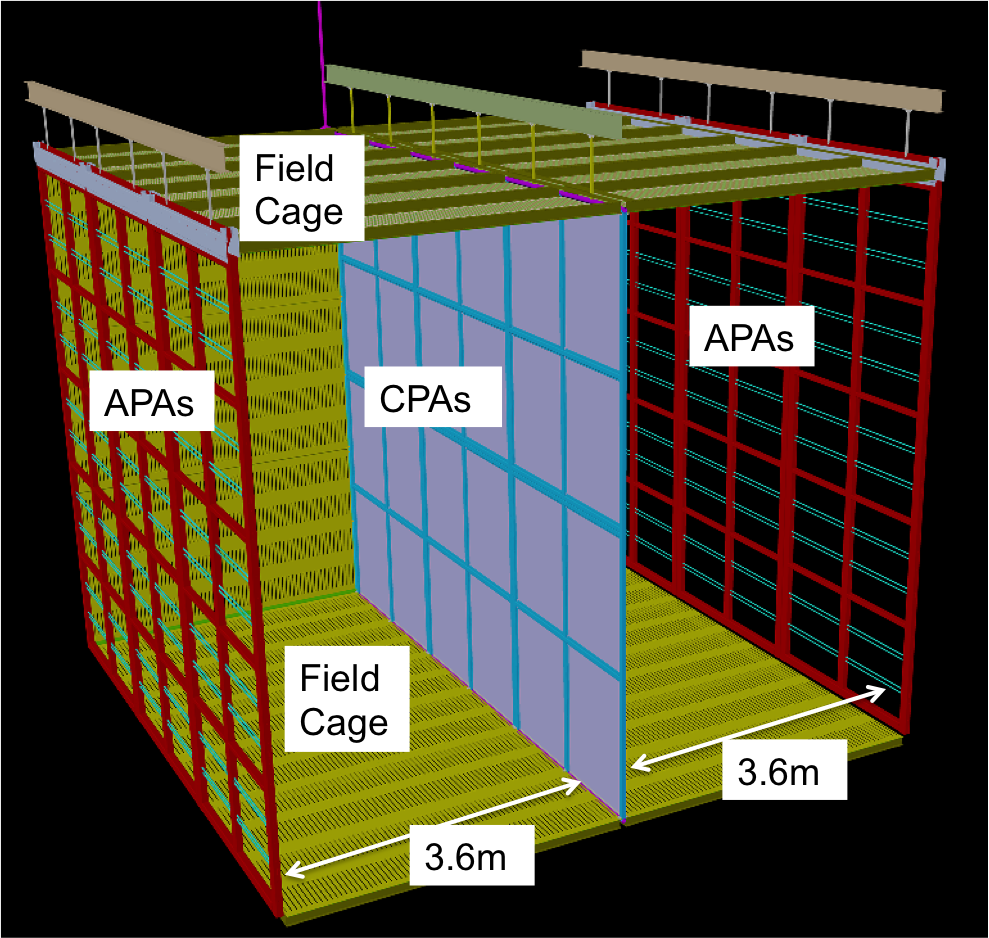
\includegraphics[width=0.40\textwidth]{CERN_single_TPC}
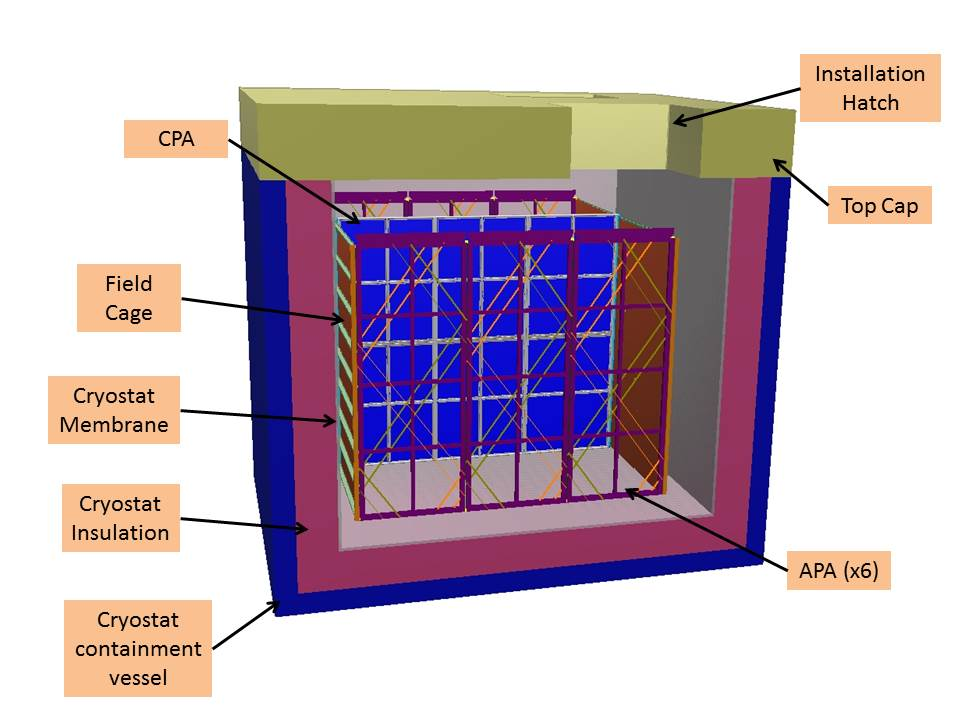
\includegraphics[width=0.59\textwidth]{TPC-3D-section}
\end{cdrfigure}
The TPC readout, photon-detection system, DAQ, slow control and
monitoring, as well as the key issues of the installation procedure
are described in corresponding sections of
Chapter~\ref{ch:detectors-fd-ref}.

\subsubsection{Cryostat}

The CERN prototype uses a membrane tank technology with internal
dimensions of 7.8~m (tranverse) $\times$ 8.9~m (parallel) $\times$ 8.1~m
(height).  It contains 725 tons of LAr, equivalent to about
520~m$^3$ (where the remaining volume contains the gas ullage). 
The active (fiducial) detector mass of LAr amounts to
400~tons (300~tons).  The external cryostat dimensions are 10.6~m
(tranverse) $\times$ 11.7~m (parallel) $\times$ 10.9~m (height).

The cryostat design is scaled up from the 35-t prototype
cryostat\cite{bib:membcryo1573}, described in
Section~\ref{sec:proto-35t}.  Unlike the 35-t cryostat, it uses a
steel outer supporting structure with an inside metal liner.  It is
similar to the WA105 dual-phase prototype detector cryostat and to
that for the Fermilab Short-Baseline Near Detector
(SBND)\cite{bib:SBND}.  The support structure rests on I-beams to
allow for air circulation underneath the cryostat; this maintains the
temperature within the allowable limits.  A stainless-steel membrane
contains the LAr within the cryostat. The pressure loading of the
cryogenic liquid is transmitted through rigid foam insulation to the
surrounding outer support structure. The membrane is corrugated to
provide strain relief resulting from temperature-related expansion and
contraction. The cryostat top cap consists of the same layers as the
cryostat walls.  From the inside out, the layers include the
stainless-steel primary membrane, intermediate insulation layers and
vapor barrier; they all continue across the top of the detector
providing a leak-tight seal.  The cryostat roof is a removable steel
truss structure to which stiffened steel plates are welded from the
underside. They form a flat vapor-barrier surface onto which the roof
insulation attaches directly.


The truss structure rests on the top of the supporting structure where
a positive structural connection between the two is made in order to
resist the upward force caused by the slightly pressurized argon in
the ullage space. The hydrostatic load of the LAr in the cryostat is
carried by the floor and the sidewalls. In order to meet the maximum
deflection of 3~mm between APA and CPA and to decouple the detector
form possible sources of vibrations, the TPCs are connected to an
external bridge over the top of the plate supported on the floor of
the building. Everything else within the cryostat (electronics,
sensors, cryogenic and gas plumbing connections) is supported by the
steel plates under the truss structure.

All piping and electrical penetrations into the interior of the
cryostat are made through the top plate.  Penetrations are clustered
in one region.  The top cap has two large openings for TPC
installation, and a manhole to allow entry into the tank after the
hatches have been closed.

\subsubsection{Cryogenics System}

The main goals of the cryogenics system are to purge the cryostat
prior to the start of the operations (with argon gas in open and
closed loops), cool the cryostat and fill it with LAr.  The LAr is
continuously purified and the boil-off argon gas is captured,
recondensed and purified.  The design calls for a 10-ms electron
lifetime (30 ppt O$_2$ equivalent), a quantity that is measured by the
detector.

The LAr-receiving facility includes a storage dewar and ambient
vaporizer to deliver LAr and gaseous Ar to the cryostat. The LAr goes through
the LAr handling and purification system, whereas the gaseous Ar goes through
%the gaseous Ar 
its own purification system before entering the cryostat.  Studies are
ongoing to standardize the filtration scheme and select the optimal
filter medium for both the prototype and future detectors.

During operation, an external LAr pump circulates the bulk of the
cryogen through the LAr purification system. The nominal LAr
purification flow rate completes one full volume exchange in 5.5~days.
The boil-off gas is recondensed and sent to the LAr
purification system before re-entering the vessel.

The proposed LAr cryogenics system is based on that of the 35-t
prototype, MicroBooNE and SBND, %Short-Baseline Near Detector,
and the current plans for the DUNE single-phase far detector module.
